\apendice{Documentación de usuario}

\section{Instalación / Puesta en marcha}

Este sistema ha sido diseñado para monitorizar, de forma sencilla y en tiempo real, dos parámetros vitales del neonato: la saturación de oxígeno y la frecuencia cardíaca. Por lo tanto, el usuario, idealmente, debería ser un médico o un enfermero que sea responsable del control de estos pacientes en ambientes como hospitales o UCIs neonatales. Aunque no se ha conseguido un objetivo final lo suficientemente fiable como para ser utilizado en un entorno real, a continuación se explica, de forma clara y práctica, cómo se colocaría el sensor y cómo interpretar lo que aparece en la pantalla como si el sistema ya estuviese integrado en la incubadora.

\subsection{Paso 1: Preparación y encendido de la incubadora}

\begin{itemize}
    \item Seguir primero las instrucciones del manual de la incubadora \textit{In$^3$ator} \footnote{El manual mencionado disponible en \href{https://ayudacontenedores.org/storage/2021/11/in3ator_user_manual-v1.0-Spanish.pdf}{Ayuda Contenedores.}}(capítulo “2.5 Panel de operación”):
    \begin{itemize}
        \item Conectar la fuente de alimentación de 12V a la cuna climática.
        \item Colocar una botella de agua nueva en el humidificador (se recomienda usar agua destilada o embotellada, nunca del grifo).
        \item Conectar el cable del humidificador a la toma correspondiente.
        \item Encender la cuna usando el interruptor general.
        \item En el menú principal o avanzado, seleccionar el modo operativo deseado:
        \begin{itemize}
            \item Configurar las semanas de gestación o ajustar manualmente la temperatura y humedad (según el caso).
            \item Activar los LEDs si se desea aplicar fototerapia.
            \item Pulsar el botón “Inicio” (Aparece una vez se configuran las opciones que señala).
            \begin{figure}[H]
            \centering
            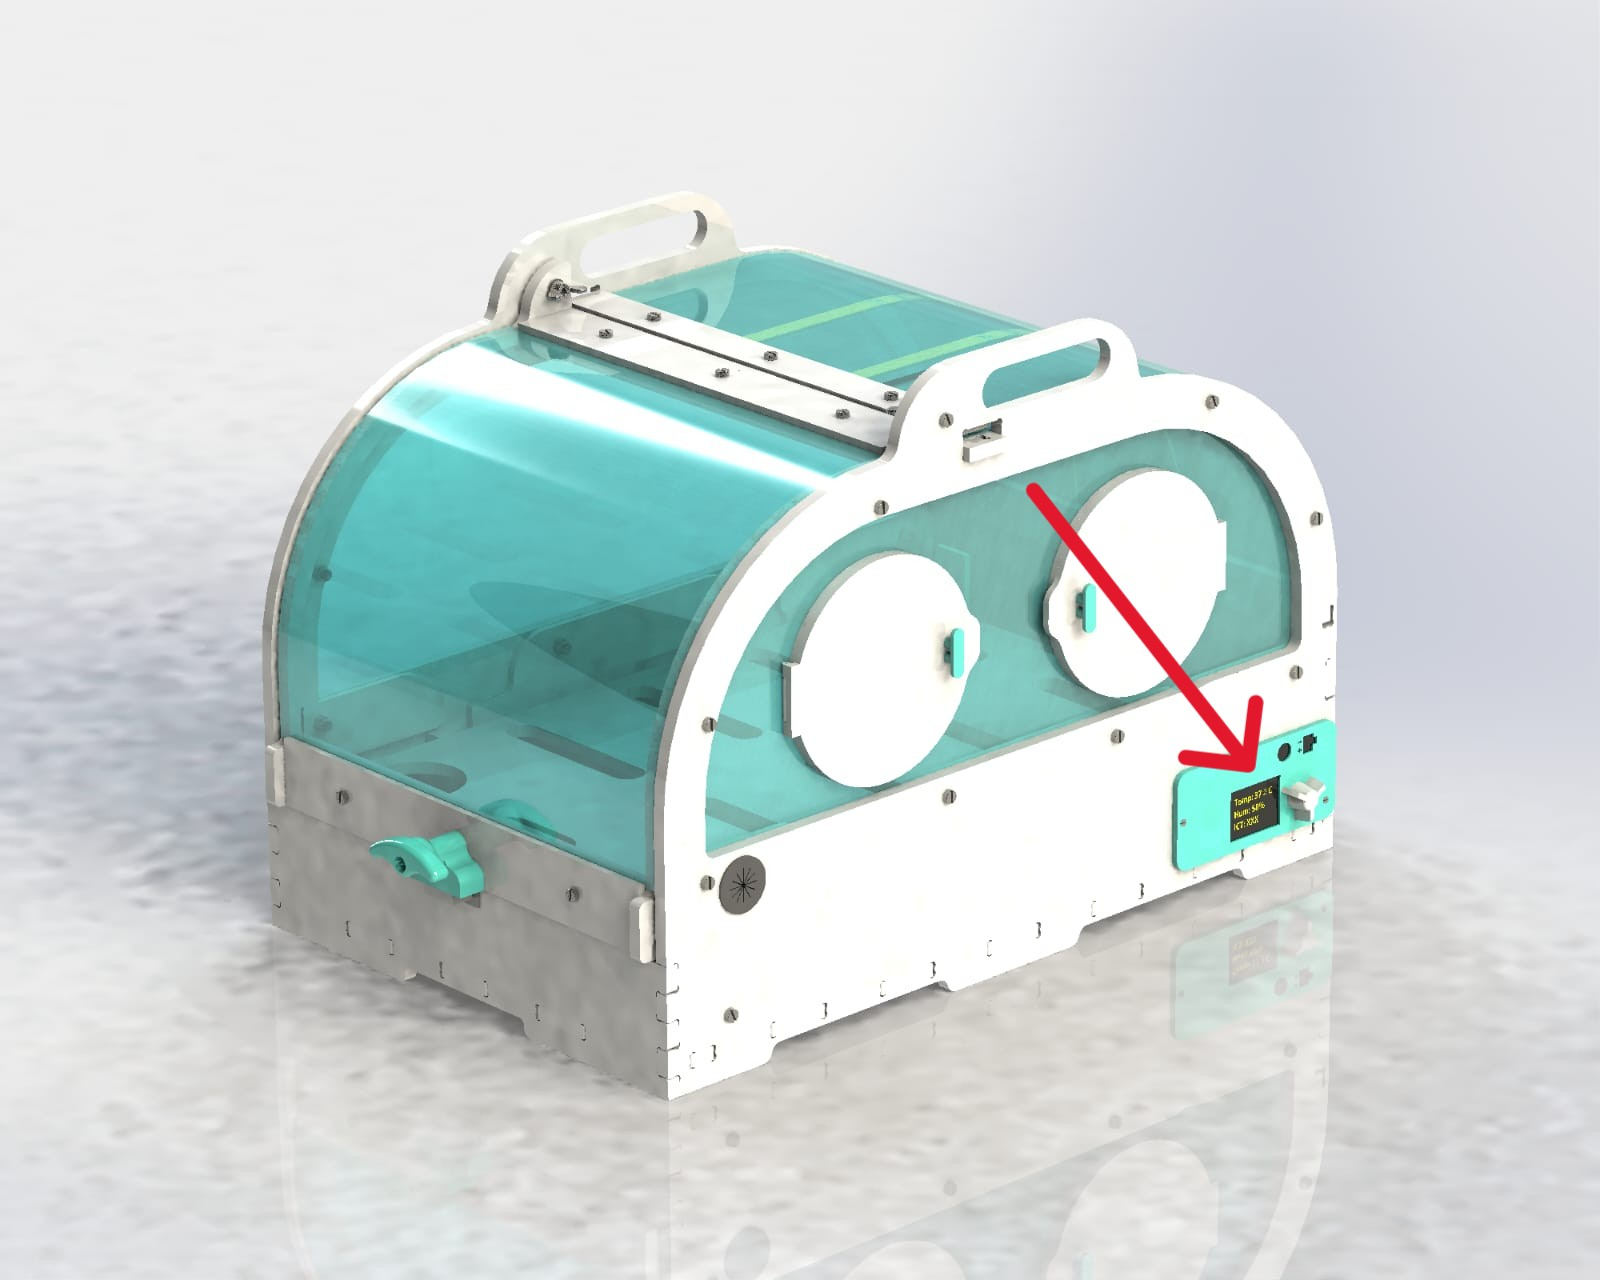
\includegraphics[scale=0.15]{img/incubadora.jpeg}
            \caption{Ubicación de la pantalla en la incubadora. Fuente adaptada: \href{https://medicalopenworld.org/la-incubadora/}{MedicalOpenWorld}}
            \label{fig:pantalla_incubadora}
            \end{figure}
    
            \begin{figure}[H]
            \centering
            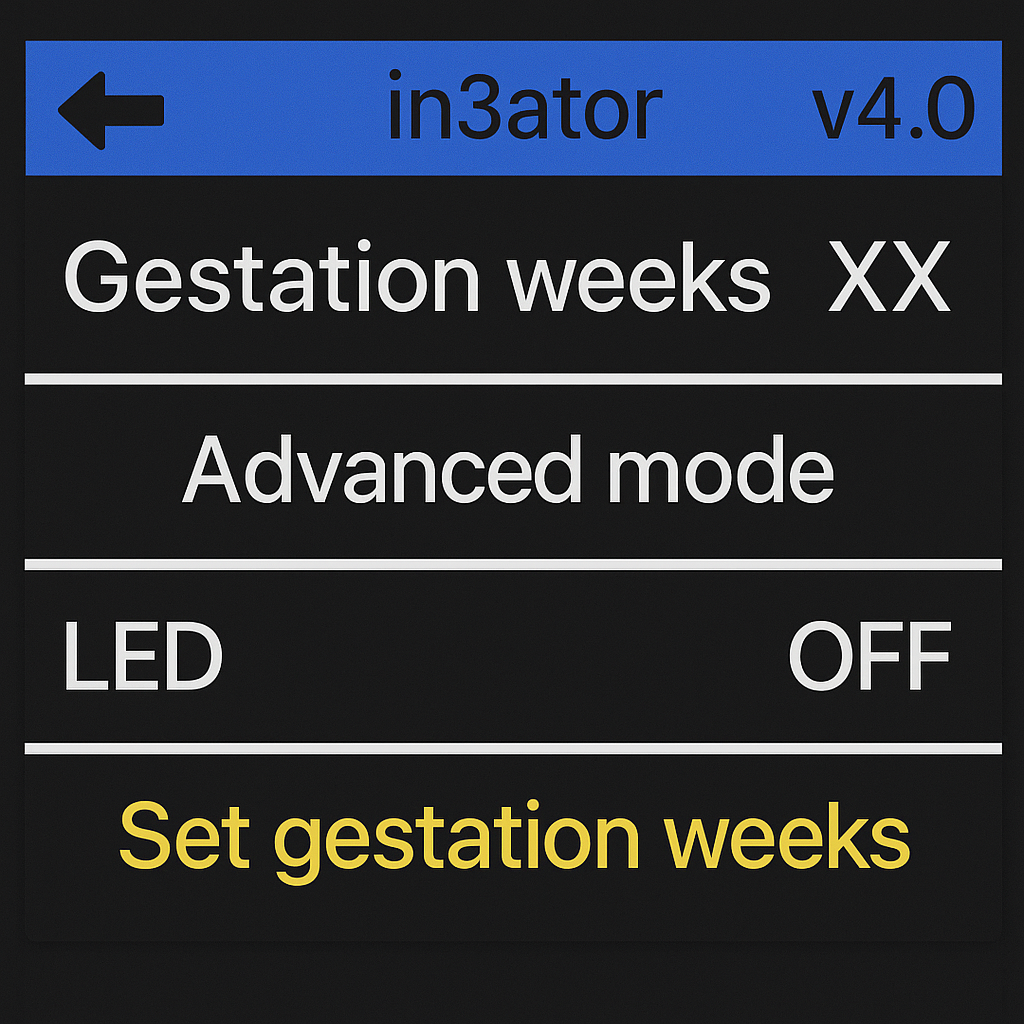
\includegraphics[scale = 0.13]{img/menu_display.png}
            \caption{Display inicial de la incubadora. Fuente adaptada: \href{https://ayudacontenedores.org/storage/2021/11/in3ator_user_manual-v1.0-Spanish.pdf}{Ayuda Contenedores.} }
            \label{fig:display}
            \end{figure}
        \end{itemize}
    \item Si es posible, dejar la cuna precalentando durante al menos 30 minutos antes de introducir al bebé.
    \end{itemize}
\end{itemize}

\subsection{Paso 2: Colocación del sensor óptico}

\begin{itemize}
    \item Antes de manipular al neonato, asegurar que la incubadora mantiene las condiciones térmicas y de humedad recomendadas.
    \item Comprobando que el sensor U401-D se encuentra bien enchufado a su puerto correspondiente, colocarlo:
    \begin{itemize}
        \item En una zona acral\footnote{La definición de “acral” es “superior” o “más alto”, y este término se refiere a una parte del cuerpo que está más alejada del centro, es decir, en los extremos de los brazos o las piernas} del paciente (pie, palma de la mano, orejas o nariz), tal como se aconseja para minimizar interferencias.
        \item Usar la cinta regulable que incluye el sensor para fijarlo sin apretar demasiado.
        \begin{figure}[H]
            \centering
            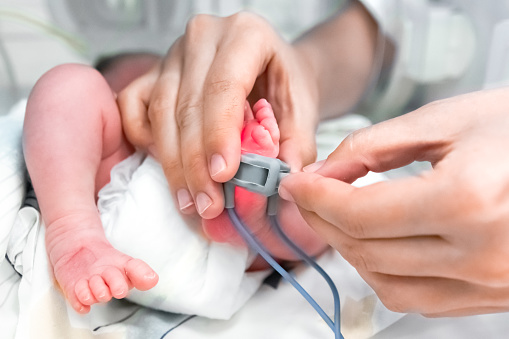
\includegraphics[width=0.4\linewidth]{img/medico.jpg}
            \caption{Ejemplo de la posición prevista para el sensor óptico. Fuente: \cite{semianovich2020oximetro}. }
            \label{fig:medico}
        \end{figure}
    \end{itemize}
\end{itemize}

\subsection{Paso 3: Visualización de los parámetros en pantalla}

\begin{itemize}
    \item En la pantalla de la incubadora, junto con los campos habituales de temperatura y humedad, se mostrará también la lectura en tiempo real de:
        \begin{itemize}
            \item Saturación de oxígeno (SpO$_2$)
            \item Frecuencia cardíaca 
            \begin{figure}[H]
            \centering
            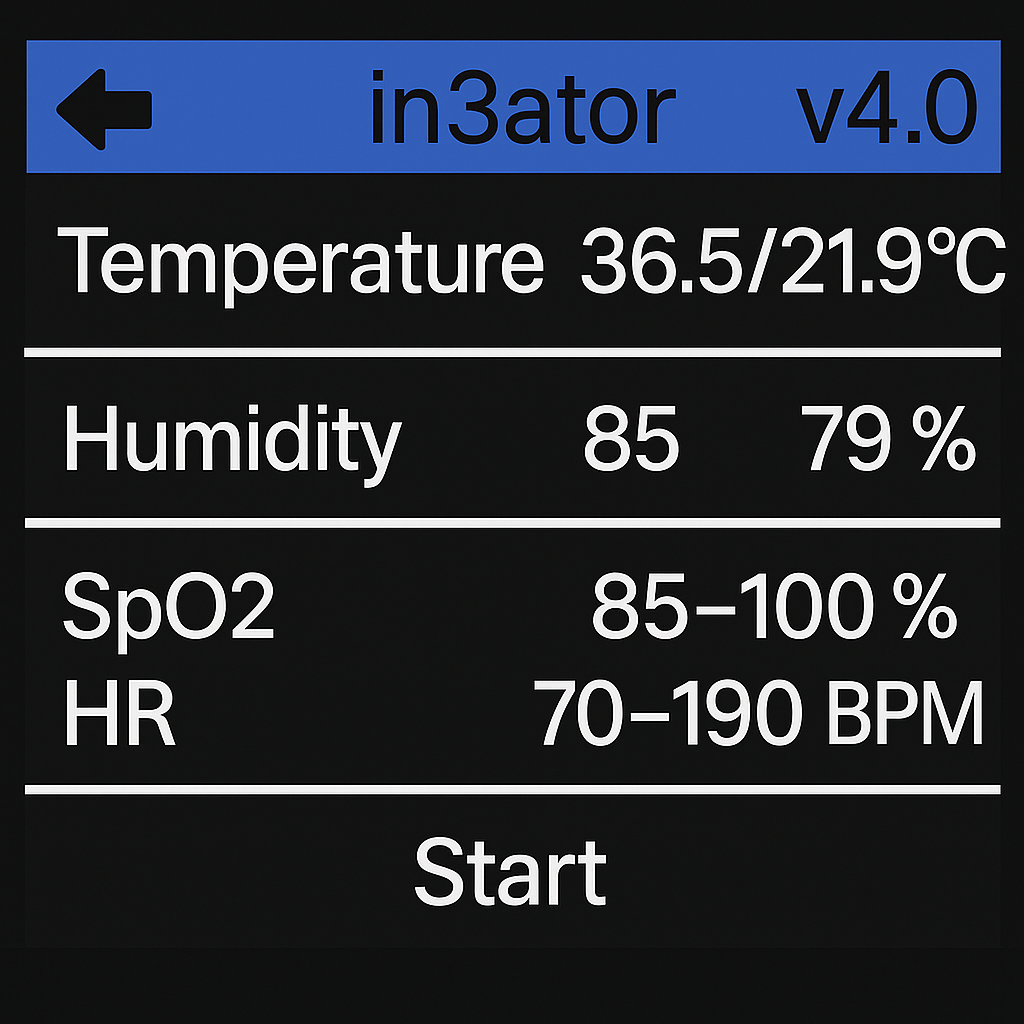
\includegraphics[scale = 0.13]{img/display.png}
            \caption{Display que muestra los parámetros que controla la incubadora. Fuente adaptada: \textit{Elaboración propia.}}
            \label{fig:display}
            \end{figure}
        \end{itemize}
    \item Estos valores pueden tardar algunos segundos en estabilizarse después de conectar el sensor.
    \item Valores normales esperados:
        \begin{itemize}
            \item \textbf{SpO$_2$:} 85–100\%
            \item \textbf{Frecuencia cardíaca:} 70-190 bpm
        \end{itemize}
    \item Si los valores se muestran inestables, parpadean, o aparecen líneas discontinuas o símbolos de error:
        \begin{itemize}
            \item Verificar que el sensor esté bien colocado.
            \item Asegurar de que el neonato esté tranquilo y que no haya movimiento excesivo.
            \item Evitar fuentes de luz intensa apuntando directamente al sensor.
        \end{itemize}
\end{itemize}

\subsection{Paso 4: Apagado del sistema o cambio de configuración}

\begin{itemize}
    \item Para detener el funcionamiento del sistema, presionar el codificador rotatorio\footnote{El codificador rotatorio es el botón giratorio situado a la derecha de la pantalla. Permite navegar por el menú girándolo, y confirmar opciones pulsándolo } durante 2 segundos (esto lleva al menú principal).
    \item Si es necesario modificar algún parámetro, acceder al modo avanzado manteniendo pulsado el codificador durante más de 5 segundos.
    \item Para apagar completamente la incubadora, desenchufar la fuente de alimentación.
\end{itemize}

\section{Manual de interpretación de los resultados obtenidos}

Los valores que muestra el sistema están diseñados para ofrecer una lectura rápida y clara del estado del neonato. En esta versión, los parámetros monitorizados son:

\begin{itemize}
    \item \textbf{SpO$_2$ (saturación de oxígeno):} se muestra como un porcentaje (\%).
    \item \textbf{HR (frecuencia cardíaca):} se muestra en pulsaciones por minuto (BPM).
\end{itemize}

\subsection{Valores de referencia esperados}

Los rangos normales pueden variar ligeramente según el estado clínico del paciente, pero en general se consideran adecuados los siguientes valores:

\begin{itemize}
    \item \textbf{SpO$_2$:} entre 85\% y 100\%. \\
    Valores por debajo de 90\% indican hipoxemia y requieren evaluación inmediata.
    
    \item \textbf{HR:} entre 120 y 160 BPM en neonatos sanos. \\
    Valores persistentemente por debajo de 100 BPM o por encima de 180 BPM pueden indicar bradicardia o taquicardia, respectivamente.
\end{itemize}


\section{Manuales y/o Demostraciones prácticas}

Aunque este anexo está enfocado a cómo podría usarse el sistema en un entorno clínico real en el futuro, también se ha incluido un vídeo complementario que muestra parte del trabajo realizado durante el desarrollo.

En el vídeo se puede ver una demostración práctica donde se compara el funcionamiento del sensor óptico conectado a la placa con un pulsioxímetro comercial. Para ello, me coloco el pulsioxímetro comercial en una mano y el sensor óptico que ejecuta el software desarrollado en la otra, y se registran los datos en tiempo real mientras se visualizan en la consola de Visual Studio Code. Esto permite comprobar que las lecturas obtenidas con ambos sistemas son similares en condiciones normales.

El vídeo está disponible en el repositorio del proyecto, en la siguiente ruta:

\begin{center}
\texttt{TFG-Elena-Ruiz/Demostraci\'on/TFG\_ElenaRuiz.mp4}
\end{center}

Este contenido no forma parte del manual clínico, pero puede ser útil para entender mejor cómo funciona el sistema y cómo se ha comprobado su comportamiento durante el desarrollo.



    
     